 \section{Graphical notations for probabilistic models}

% (COPIED FROM DAMIEN THESIS) Notations were adapted from~\cite{Dietz2010-technical-report-graphs}. The different types of model variables are represented with different types of nodes in the network; nodes repetitions are expressed with plate notations and the conditional dependency between nodes is expressed with directed arrows:
% \begin{center}
%   \begin{tabular}{m{8cm} m{2cm}}
%     Observed variables & \tikz{\node[obs](){$Y$}}\\
%     Unobserved probabilistic variables & \tikz{\node[latent](){$\theta$}}\\
%     Unobserved parameters & \tikz{\node[latent,double, double distance=1pt](){$\theta$}}\\
%     Repetition of node $\theta_n$ for $n\in\llbracket1;N\rrbracket$ & \tikz{\node[latent](theta){$\theta_n$}; \plate[] {plateN} {(theta)} {$N$};}\\
%     Conditional dependency between nodes: $P(Y,\theta) = P(Y|\theta)P(\theta)$ & \tikz{%
%             \node[latent]   (theta) {$\theta$};
%             \node[obs, xshift=1.5cm] (Y) {$Y$};
%             \edge{theta}{Y}}
%   \end{tabular}
% \end{center}
% For simplicity, fixed hyperparameters are not represented on the graphical model. Unobserved parameters are only represented when optimised together with the unobserved probabilistic variables.

\section{Latent variable models for genomics}
With the exponential growth in the use of high-throughput genomics, biological data sets are increasingly high dimensional, both in terms of samples and features. A key principle of biological data sets is that variation between the measured features result from differences in underlying, often unobserved, processess. Such hidden processess, whether biological or technical, affect multiple features in a coordinated fashion due to the existence of interacting gene regulatory networks. This key assumption sets off an entire statistical framework of exploiting the redundancy encoded in the data set to learn the (latent) sources of variation in an unsupervised fashion. This is the aim of dimensionality reduction techniques, or latent variable models (LVMs) \cite{Komili2008, Leek2007, Pournara2007, Dai2017, Genevieve2018, Meng2016}.

\subsection{General mathematical formulation}
Given a dataset $\bfY$ of $N$ samples and $D$ features, LVMs attempt to explain the observations by means of a potentially smaller set of $K$ latent variables, or factors. The mapping between the low-dimensional and the high-dimensional space is performed via a function $f(\bfX|\bTheta)$ that depends on some parameters $\bTheta$.\\

The choice of $f(\bfX|\bTheta)$ is essentially the field of dimensionality reduction. A trade-off exists between complexity and interpretation. While non-linear functions such as deep neural autoencoders provide more explanatory power\cite{}, this leads to a considerable challenge in interpretation. Hence, for most applications where interpretability is important, $f(\bfX|\bTheta)$ is assumed to be linear:
\begin{equation} 
	y_{nd} = \sum_{k=1}^{K} w_{dk}z_{n,k}
\end{equation}
or in matrix form:
\begin{equation} \label{eq:linear_model}
	\mathbf{Y} = \mathbf{Z}\mathbf{W}^{T}
\end{equation}
where $\bfZ \in \R^{N \times K}$ is a matrix that contains the factors (and hence $K<D$). The matrix $\bfW \in \R^{D \times K}$ contains the weights or loadings, which provide the linear mapping between the high-dimensional space (the features) and the low-dimensional space (the latent factors).\\
Note that the aim of the model is to capture the coordinated heterogeneity between features, not to explain differences in their total levels, and hence features are assumed to be centered.\\

The inference procedure consists in learning the values of all unobserved variables, including latent variables and the weights. As we shall demonstrate, different inference schemes and assumptions on the prior distributions lead to significantly different model outputs.

\subsection{Principal component Analysis}
Principal Component Analysis (PCA) is the most popular technique for dimensionality reduction \cite{Hotelling1933,Ringner2008}.\\
Starting from \Cref{eq:linear_model}, two formulations of PCA exist \cite{Bishop}. In the maximum variance formulation, the aim is to infer an orthogonal projection of the data onto a low-dimensional space such that variance explained by the projected data is maximised. For a single principal component, the optimisation problem is:
\begin{align} \label{eq:pca}
	\argmax_{\|\bfw\|=1} & \sum{n=1}^{N} (\bfw_1^T \bfy_n)^2 \\
						 & \bfw_1^T \bfX^T \bfX \bfw \\
						 & \bfw_1^T \bfS \bfw
\end{align}
where $\bfS \in \R^{D \times D}$ is the data covariance matrix defined as $\bfS = \bfX^T \bfX$. The mapping between the high-dimensional space and the low-dimensional space is done again via a vector of loadings $\bfw_1^T$. \\
The $k$-th principal component can be found by subtracting the reconstructed data by the previous $k-1$ principal components from $\bfY$. If we define $\bfz_k=(\bfw_k^T \bfY)$ to be the $k$-th principal component, the optimisation problem is:
\[
	\hat{\bfY} - \bfY - \sum_{k=1}^{K} (\bfz_k \bfw_k^T)
\]
and re-applying \Cref{eq:pca}\\

In its minimum error formulation, the aim is to find an equivalent projection that minimises the mean squared error between the observations and the reconstruction:
\[
	\argmax_{\|\bfw\|=1} \| \bfY - \sum_{k=1}^{K} \bfz_k \bfw_k^T \|^2
\]

% Nice figure here:
% 	http://alexhwilliams.info/itsneuronalblog/2016/03/27/pca/

Solving the two optimisation problems above via Lagrange multipliers leads, remarkably, to the same solution\cite{Bishop}:
\begin{equation}
	\bfS \bfw_k = \lambda_k \bfw_k
\end{equation}
Hence, the loading vectors $\bfw_k$ are equivalent to the eigenvectors of $\bfS$, which can be computed via singular value decomposition.

(EXPLAIN WHY THE TWO SOLUTIONS ARE THE SAME) \\

 
The main strength of PCA relies on its simplicity and closed form solution. Additionally, the linear mapping has the advantage of yielding interpretable loadings, so that inspection of $\bfw_k$ reveals which features are jointly affected by the $k$-th principal component.\\
However, PCA suffers from serious drawbacks when applying it to real data sets. First, biological measurements are inherently noisy, and there is no explicit account of noise in PCA. In practice, high variance components are often asociated with signal whereas low-variance components are assumed to be noise, but an ideal model should explicitly disentangle the uncoordinated (or unexplained) variability that is attributed to noise from the coordinated variability that is characterised as signal. Second, in its original formulation, no missing data is allowed. Third, there is no rationality on how to evaluate the fit and perform model selection. Finally, it does not offer a principled way of modelling prior information about the data.

\subsection{Probabilistic Principal Component Analysis and Factor Analysis}

A generalisation of PCA can be achieved by converting the equation \Cref{eq:linear_model} into a probabilistic framework with an explicit noise term\cite{TippingBishop}:
\begin{equation}
	\bfY = \bfW \bfZ + \bepsilon
\end{equation}
where the weights $\bfW$ are assumed to be fixed parameters. In contrast, the noise $\bepsilon$ and the latent variables $\bfZ$ (the principal components) are assumed to be normally distributed random variables (\cref{fig:pPCA}):
\begin{align}
	p(z_{nk}) &= \Ndist{z_{nk}}{0,1} \\
	p(\epsilon) &= \Ndist {\epsilon}{0,\sigma^2}
\end{align}

All together, this leads to a normally-distributed likelihood:
\begin{equation}
	p(\bfY|\bfW,\bfZ,\sigma) = \Ndist{\bfY}{\bfW \bfZ,\sigma^2 \I}
\end{equation}

\begin{figure}[H] \begin{center}
	% \definecolor{colD}{rgb}{0.2, 0.2, 0.6}
\definecolor{colM}{rgb}{0.0, 0.5, 0.0}
\definecolor{colN}{rgb}{0.5, 0.0, 0.13}
\definecolor{colG}{rgb}{1.0, 0.65, 0.0}
\newcommand\op{0.25}
\colorlet{shadecolor}{black!25}


\begin{tikzpicture}

% Define nodes
\node[obs]   (Y) {$y_{n,d}$};
\node[latent, xshift=-1.5cm, above=of Y, yshift=-0.4cm] (Z) {$z_{n,k}$};
\node[latent, double, double distance=1pt, above=of Y, yshift=0.6cm] (W) {$w_{d,k}$};
\node[latent, double, double distance=1pt, xshift=1.5cm] (Tau) {$\tau$};

% Connect the nodes
\edge {Z,W, Tau} {Y};

% Plates
\plate[] {plateK} {(Z)(W)} {$K$};
\plate[] {plateN} {(Y)(Z)(plateK.south east)(plateK.south west)} {$N$};
\plate[] {plateD} {(Y)(W)(plateK.north east)(plateN.south east)} {$D$};

\end{tikzpicture}
	\label{fig:pPCA}
	\caption{Graphical model for probabilistic PCA. The latent variables are modelled as random variables, whereas the loadings and the noise are modelled as deterministic parameters.}
\end{center} \end{figure}

Importantly, The choice of the distribution for $\epsilon$ implies that the noise of each feature is independent but restricted to have the same magnitude. In practice, this is a limiting assumption, as different features are expected to show different levels of noise. This assumption can be easily relaxed and forms the basis of (probabilistic) Factor Analysis \cite{???}.\\

The inference procedures involves learning the parameters $\bfW$, and $\sigma^2$ and a posterior probability distribution for $\bfZ$.\\
In models that depend on unobserved latent variables, inference can be performed using the iterative Expectation-Maximisation (EM) algorithm \cite{Rubin1983}. In the expectation step, the posterior distribution for $\bfZ$ is computed in closed form (due to conjugacy between the likelihood and the prior), given current estimates for the parameters $\bfW$, and $\sigma^2$. In the maximisation step, the parameters are calculated by maximising the expectation of the joint log likelihood under the posterior distribution of $\bfZ$ found in the E step \cite{TippinBishop}.

Interestingly, the authors showed that the EM solution of probabilistic PCA lies in the same subspace than the traditional PCA solution \cite{ppca}. Yet, the use of a probabilistic framework brings several benefits. First, model selection can be performed by comparing likelihoods across different settings of parameters. Second, missing data can naturally be accounted for by ignoring the missing observations from the likelihood. Finally, the probabilistic formulation sets the core framework for a Bayesian treatment of PCA, enabling a broad range of principled extensions tailored different types of data sets.


\subsection{Bayesian Principal Component Analysis and Bayesian Factor Analysis}

The full Bayesian treatment of PCA requires the specification of prior probability distributions for all unobserved variables:
\begin{align}
	p(z_{nk}) &= \Ndist{z_{nk}}{0,1} \\
	p(w_{dk}) &= \Ndist{w_{dk}}{0,1} \\
	p(\epsilon) &= \Ndist {\epsilon}{\tau} \\
	p(\tau) &= \Gamma{\tau}{a_0,b_0}
\end{align}
where $\tau$ is the precision (inverse of the variance) of the noise term. A generalisation to bayesian Factor Analysis follows by allowing a separate noise term per feature:
\begin{align}
	p(\tau_d) &= \Ndist {\epsilon_d}{0,\tau_d^2} \\
	p(\tau_d) &= \Gamma{\tau_d}{a_0,b_0}
\end{align}
where $a_0$ and $b_0$ are fixed hyperparameters. This results in the following likelihood:
\[
	p(\bfY|\bfW,\bfZ,\btau) = \prod_{n=1}^{N} \prod_{d=1}^{D} \Ndist{y_{nd}}{\bfw_{d,:}^T \bfz_{n,:},\tau_d}
\]

\begin{figure}[H] \begin{center}
	\begin{tikzpicture}

% Define nodes
\node[obs]   (Y) {$y_{n,d}$};
\node[latent, above=of Y, xshift=-1.5cm] (Z) {$z_{n,k}$};
\node[latent, above=of Y, xshift=1.5cm] (W) {$w_{d,k}$};
\node[latent, xshift=1.5cm] (Tau) {$\tau_{d}$};

% Connect the nodes
\edge {Z,W, Tau} {Y};

% Plates
\plate[] {plateK} {(Z)(W)} {$K$};
\plate[] {plateN} {(Y)(Z)(plateK.north west)} {$N$};
\plate[] {plateD} {(Y)(W)(Tau)(plateK.south east) (plateN.south east) (plateN.north east)} {$D$};

\end{tikzpicture}
	\label{fig:bayesianFA}
	\caption{Graphical model for bayesian Factor Analysis. All unobserved variables are modelled as random variables.}
\end{center} \end{figure}

\subsubsection{Hierarchical priors: Automatic relevance determination}
A key advantage of the full Bayesian treatment, as opposed to the probabilistic PCA model, is that it explicitly captures uncertainity on the estimation of all unobserved variables. Yet, more importantly, the use of (hierarchical) prior distributions allow different modelling assumptions to be encoded, thereby providing a flexible and principled approach to address the limitations of PCA.\\

For example, a major challenge in PCA is how to determine the dimensionality of the latent space (i.e. the number of principle components). The use of hierarchical prior distributions allows the model to introduce sparsity assumptions on the loadings such that only a small subset of (active) factors will contain non-zero leadings.\\
In the context of Factor Analysis, the Automatic Relevance determination (ARD) prior was one of the first ones to be proposed \cite{(David J. C. MacKay, 1994; Neal, 1995; Wipf and Nagarajan, 2008)}:
\begin{equation*} \label{eq:ard}
	P(\bfW|\balpha) = \prod_{k=1}^{K} \Ndist{\bfw_{:,k}}{0,\frac{1}{\alpha_{k}}\I_{D}}\\
	\qquad\qquad
	P(\balpha) = \prod_{k=1}^{K} \Gdist{\alpha_k}{a_0^\alpha, b_0^\alpha}\\
\end{equation*}
The aim of this prior is two-fold. First, the zero-mean normal distribution specifies that, \textit{a priori}, no information is available and all features are inactive. When exposed to some data, the posterior distribution for $\bfW$ will be estimated by weighting the contribution from the likelihood and from the prior, hence allowing each feature to escape from the initial zero.\\
Second, performing inference on the variable $\balpha$ enables the model to automatically learns the number of factors. To understand this, let us assume that only $K=5$ true factors exist, but the model is initialised with $K=20$ factors. In such case, inactive factors can be prunned out by driving the corresponding $\alpha_k$ to infinity. In turn, this causes the posterior $p(\bfW_{:,k}|\bfY)$ to be sharply peaked at zero \Cref{fig:ard}, resulting in the full inactivation of all loadings \Cref{fig:hinton}. 

\begin{figure}[H] \begin{center}
	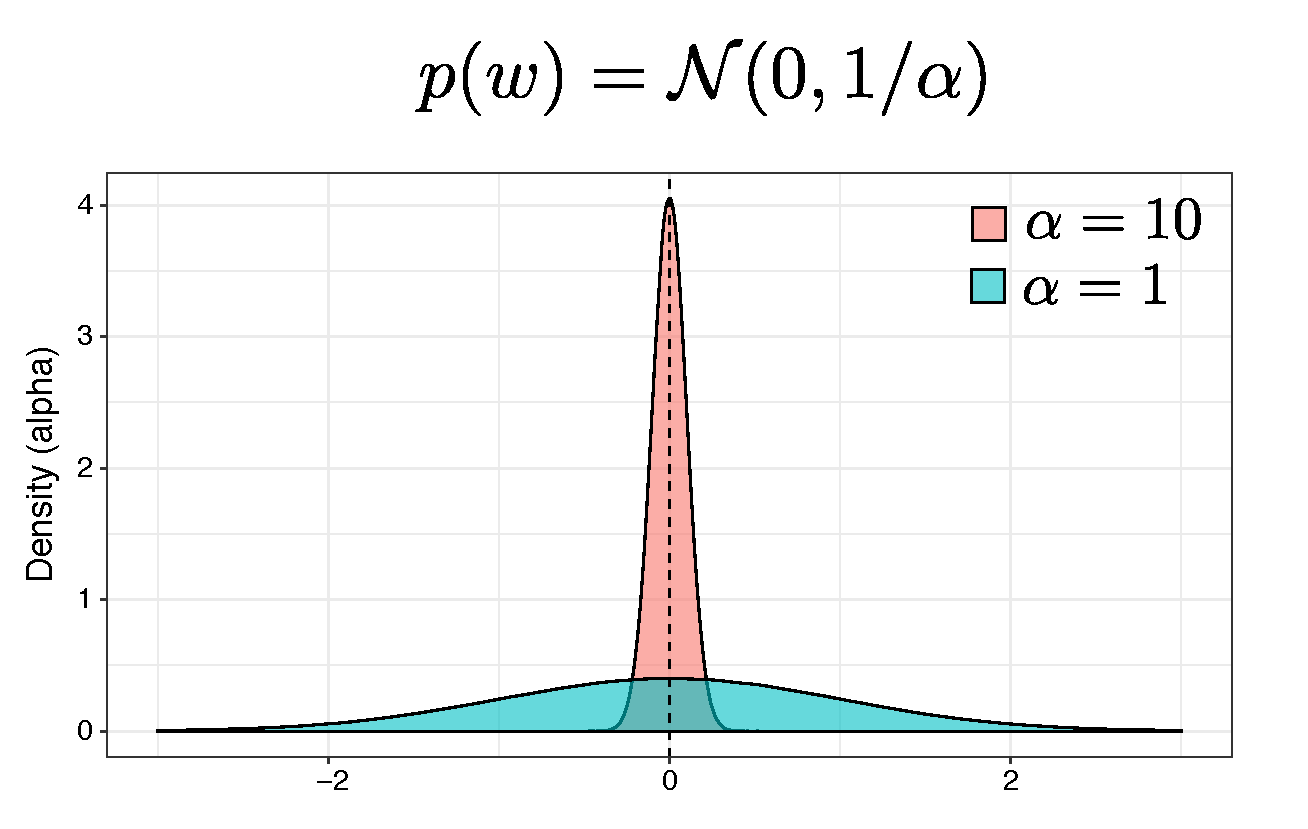
\includegraphics[width=0.8\textwidth]{Chapter2/Figs/ard}
	\caption{}
	\label{fig:ard}
\end{center} \end{figure}

\begin{figure}[H] \begin{center}
	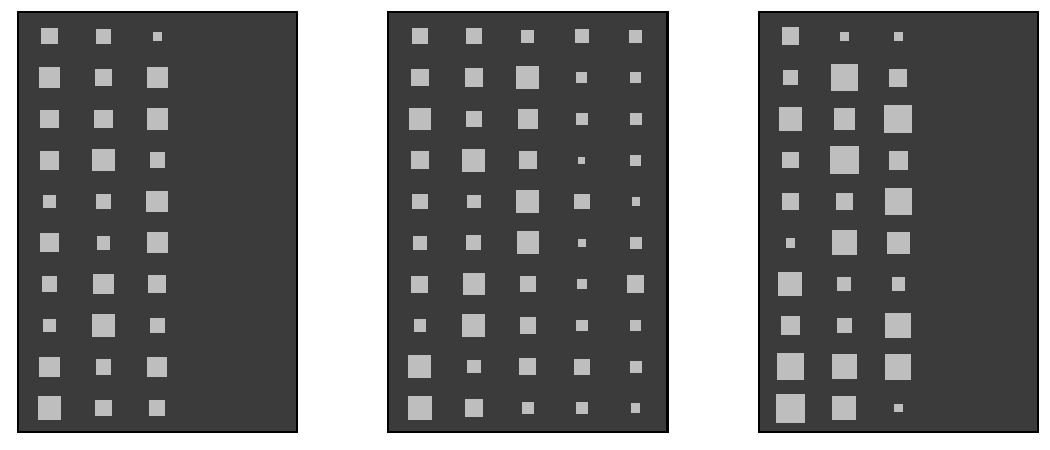
\includegraphics[width=0.8\textwidth]{Chapter2/Figs/hinton}
            \caption[Hinton plot of the loading matrix for a bayesian Factor Analysis model with an ARD prior]{Hinton plots display the values of the loading matrix, similar to a heatmap, where bigger squares depict larger loadings. Shown are the Hinton plots for (a) the true weights, (b) the infered weights by a Factor Analysis model with no ARD prior (middle), and (c) the infered weights by a Factor Analysis model with ARD prior per factor.\\
            This figure was generated using simulated data with $N=100$ samples, $D=10$ features and $K=3$ factors.}
	\label{fig:hinton}
\end{center} \end{figure}

\subsubsection{Hierarchical priors: Spike-and-slab prior}
Sparse extensions of the Bayesian factor analysis model have been proposed as a regularisation mechanism but also to model inherent assumptions regarding the sparse nature of biological data \cite{West2003,Stegle2012,Gao2013}. In practice, the variability observed in biological data sets is driven both by strong technical factors (i.e. batch effects) and by relatively weak biological factors, driven by potentially small gene regulatory networks \cite{Gao2013}. Hence, a realistic factor analysis model should be learn both types of factors. The ARD prior proposed in \Cref{eq:ard} allows entire factors to be dropped out from the model, but it provides a weak degree of regularisation in the feature loadings of active factors.\\
A sparse generalisation of the bayesian Factor Analysis model can be achieved by combining the ARD prior with a spike-and-slab prior \cite{(Mitchell and Beauchamp, 1988) }:
\begin{equation}
	p(w_{d,k} \mid \alpha_k,\theta_k) = (1-\theta_k) \mathds{1}_0(w_{d,k}) + \theta_k \Ndist{w_{d,k}}{0, \alpha_k^{-1}}
\end{equation}

\begin{figure}[H] \begin{center}
	\begin{tikzpicture}

% Define nodes
\node[obs]   (Y) {$y_{n,d}$};
\node[latent, above=of Y, xshift=-1.5cm] (Z) {$z_{n,k}$};
\node[latent, above=of W, xshift=-0.75cm] (Theta) {$\theta_{k}$};
\node[latent, above=of W, xshift=0.75cm] (Alpha) {$\alpha_{k}$};
\node[latent, above=of Y, xshift=1.5cm] (W) {$w_{d,k}$};
\node[latent, xshift=1.5cm] (Tau) {$\tau_{d}$};

% Connect the nodes
\edge {Theta, Alpha} {W};
\edge {Z, W, Tau} {Y};

% Plates
\plate[] {plateK} {(Z)(W)(Theta)(Alpha)} {$K$};
% \plate[] {plateN} {(Y)(Z)(plateK.north west)} {$N$};
\plate[] {plateN} {(Y)(Z)} {$N$};
\plate[] {plateD} {(Y)(W)(Tau)(plateK.south east) (plateN.south east) (plateN.north east)} {$D$};

\end{tikzpicture}
	\label{fig:bayesianFA}
	\caption{Graphical model for bayesian sparse Factor Analysis}
\end{center} \end{figure}

The spike-and-slab prior is effectively a mixture model where features are sampled from a zero-inflated gaussian distribution, where $\theta \in (0,1)$ dictates the level of sparsity (i.e. how many active features). A value of $\theta_k$ close to $0$ implies that most of the weights of factor $k$ are shrinked to $0$ (i.e. a sparse factor), whereas a value of $\theta_k$ close to $1$ implies that most of the weights are non-zero (i.e. dense factors). Hence, by learning $\theta_k$ from the data, the model naturally accounts for combinations of sparse and dense factors. As in \Cref{eq:ard}, $\alpha_k$ provides the ARD regularisation required to prune inactive factors. \\


\subsubsection{Inference}
In a fully Bayesian setting, the inference procedure corresponds to learning the posterior distributions for each unobserved variable. However, applying Bayes rule yields an analytically intractable solution, and approximate methods are required. This is discussed in Chapter X.
